\documentclass[final,a4paper]{article}
\usepackage[utf8]{inputenc}
\usepackage{amsmath}
\usepackage{graphicx}
\usepackage{url}
\usepackage{fancyhdr}
\usepackage{datetime}

\newcommand{\course}{Operating Systems, 5dv171}
\newcommand{\semester}{Fall 2017}
\newcommand{\assignment}{Project Linux Kernel Module - part 1}
\newcommand{\authors}{
  Igor Ramazanov, ens17irv@cs.umu.se\\
  Erik Ramos, c03ers@cs.umu.se\\
  Bastien Harendarczyk, ens17bhk@cs.umu.se\\
  \vspace{1em}
}
\newcommand{\lecturer}{Jan Erik Moström}
\newcommand{\assistants}{Adam Dahlgren}
\newcommand{\codebase}{https://git.cs.umu.se/c03ers/5dv171-project}

\setlength{\parindent}{0em}
\setlength{\parskip}{1em}

\title{
  \vspace{4em}
  \pagenumbering{gobble}
  \begin{center}
  {\LARGE \bf \course{}, \semester}\\
  {\Large \bf \assignment}\\
  \vspace{6em}
  {\normalsize
  {\bf Teacher}\\
  {\lecturer}\vspace{1em}\\
  {\bf Teaching assistant}\\
  {\assistants}\vspace{1em}\\
  {\bf Group members}\\
  \authors
  {\bf Gitlab repository}\vspace{-1em}\\
  {\codebase}}
  \end{center}
}

\author{}
\date{}
\pagestyle{fancy}
\fancyhead[R]{\the\year-\twodigit{\the\month}-\twodigit{\the\day}}
\renewcommand{\headrulewidth}{0em}

\begin{document}
\maketitle
\pagebreak
\pagenumbering{arabic}

\begin{figure}
  \centering
  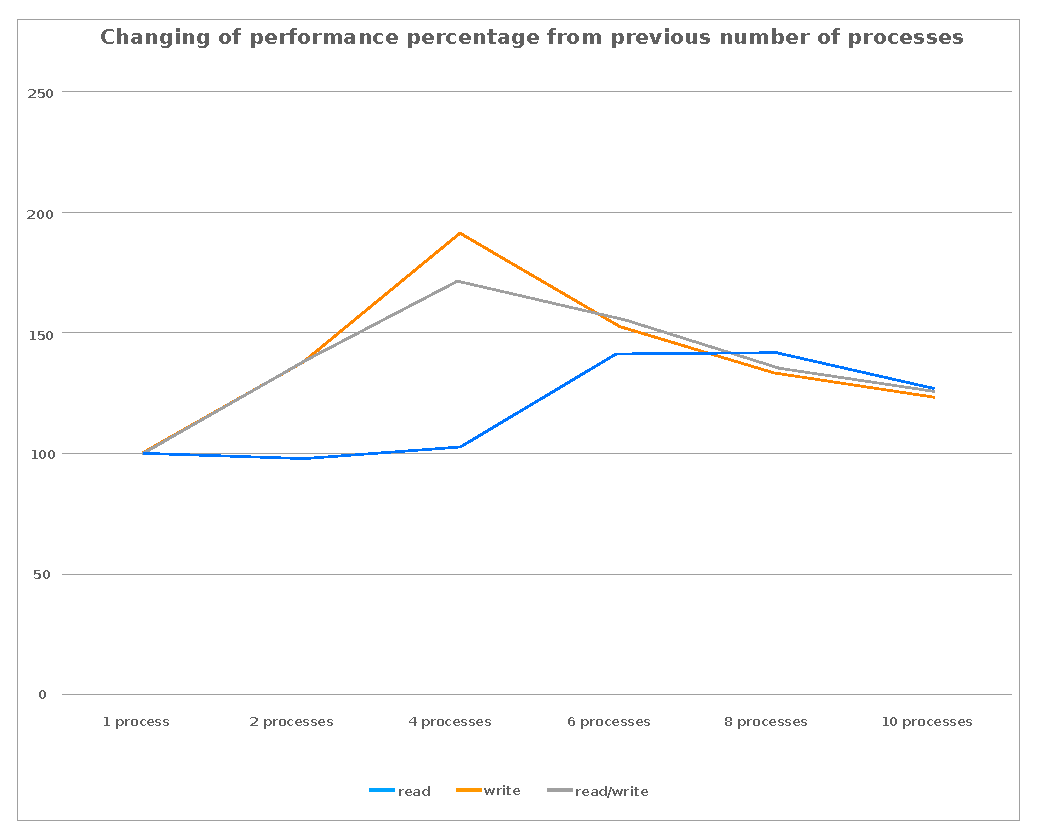
\includegraphics[scale=.7]{percentages.eps}
\end{figure}

\begin{figure}
  \centering
  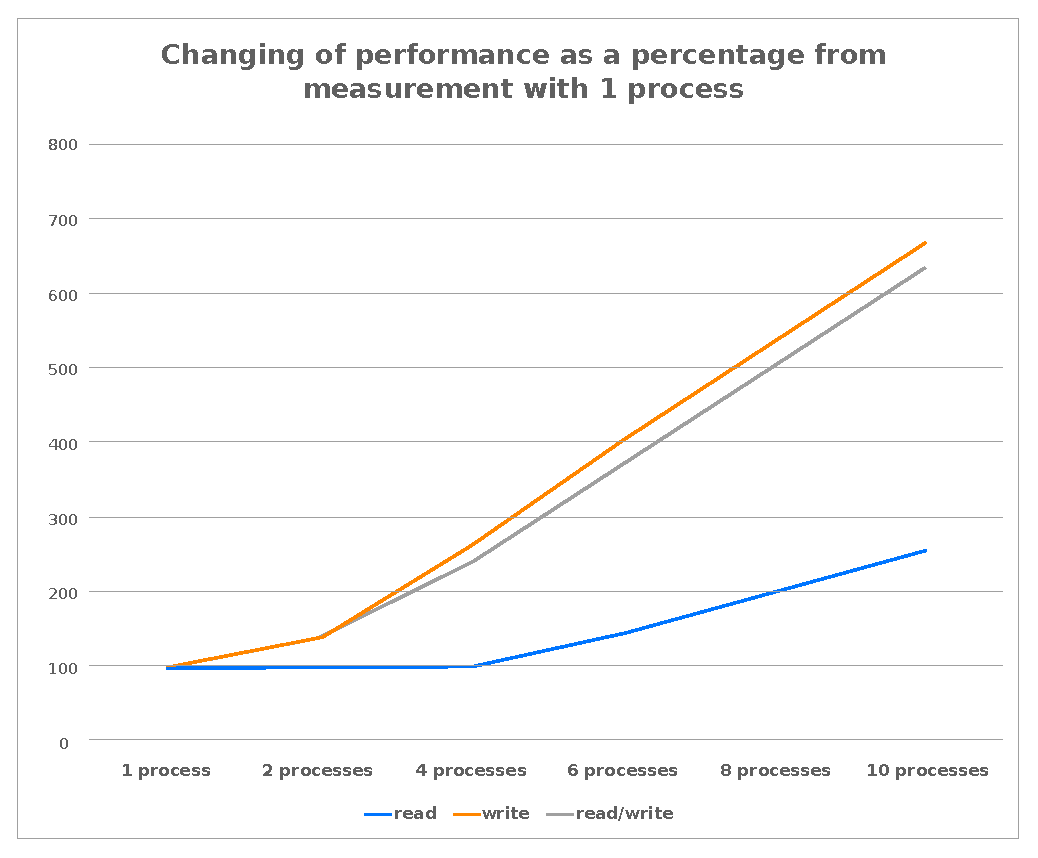
\includegraphics[scale=.6]{percentages1.eps}
\end{figure}

\begin{tabular}{|l|l|l|l|l|l|l|}
  \hline
  & 1 process & 2 processes & 4 processes & 6 processes & 8 processes
  & 10 processes \\
  \hline
  read & 0.926 & 0.897 & 0.928 & 1.316 & 1.861 & 2.63 \\
  \hline
  write & 3.082 & 4.223 & 8.076 & 12.371 & 16.568 & 20.563 \\
  \hline
\end{tabular}

\section*{User's guide}
The project consists of two parts - the kernel module and the user space
test program. All files required to build both parts can be found in the gitlab
repository.

To build the project, begin by cloning the repository typing the following in
a terminal:
\begin{center}
{\tt git clone \codebase}
\end{center}
In the project directory there are two sub directories; module and program.
Both of these directories have a Makefile for building. Simply enter the
directories and type {\tt make} in the terminal.

Once built, a super-user may install the module by typing 
{\tt insmod moddb.ko} in the terminal and later {\tt rmmod moddb}
to uninstall it.

The test program \emph{test}, can be used both for putting data
into the module and to retrieve data from it. Inserting data is done like this:
\begin{center}
{\tt ./test set key value}
\end{center}
To retrieve data from the module using the test program, instead write this:
\begin{center}
{\tt ./test get key}
\end{center}

\section*{Problem description}
The goal with this project is to write a Linux Kernel Module (LKM) that allows
different processes running on the same Linux machine, to access shared data
through key-value mappings, stored in the kernel. The system must be robust
enough, that multiple processes, running on multiple processors, can use it
without accidentally corrupting the stored data. A user space application must
also be implemented to demonstrate the functionality of the LKM.

This first part of the project report describes how the LKM represents these
mappings, how the user space applications communicate with the module and
what considerations went into the decisions.\pagebreak

\section*{Solution}
The following three methods of user to kernel space communication were
considered for this project:
\begin{enumerate}
  \setlength\itemsep{0em}
  \item Device files
  \item Proc files
  \item Netlink sockets
\end{enumerate}
Using one of the file systems to solve the problem was appealing, primarily
because much of the heavy lifting would be done by system calls already
available in Linux. However, since device files usually represent actual,
physical devices and proc files are meant to contain information about
processes, none of these seemed like a really good fit.

Because the kernel module would provide user space applications with a service,
in much the same way that an Internet server would to its clients, Netlink
sockets seemed like a much better fit. They would however, turn out to be much
more complicated to set up and use.

When it came to storing the key-value pairs in the module, there were two
options available; to make a new hashtable datatype, or to find an existing
one to use. Not a difficult choice.

A hashtable datatype called \emph{rhashtable} is provided by the
Linux kernel and offers all the basic hashtable functionality required
at a this stage of the project. It is also designed to run well in
multi-threaded environments, which will come in handy later in the project.

\section*{Discussion}
Developing for the Linux kernel is not an easy task. Much of the information
available online is outdated and the kernel in many places, is poorly
documented. Most of the time spent on the project, was dedicated to sifting
through kernel code, trying to to figure out what the functions do, which
functions to use and in what contexts they are safe to use.

Debugging is also difficult, in part because many tools run only in user space.
Another complicating factor, is the fact that the operating system can freeze
when there is a bug in the code and that error print-outs are lost when
rebooting.
\end{document}
